In this Section, we establish the preliminary notations and introduce the
mathematical models that will be used throughout the paper.

\subsection{Measurement Representation}
A nodding laser range-finder produces scan measurements $\mathbf{s}_i=[r_i,
\theta_i,\psi_i]^\text{T}$ that are transformed into their corresponding
Cartesian 3D coordinates $\mathbf{p}_i=[x_i,y_i,z_i]^\text{T}$, where $r_i$ is
a range measurement, $\theta_i$ a pitch angle, and $\psi_i$ a bearing angle. The
sensing device has an error model which is typically a function of
$\mathbf{s}_i$. From a complete laser sweep, we obtain a point cloud
representation $\mathcal{P}=\{\mathbf{p}_1,\mathbf{p}_2,\dots,\mathbf{p}_N\}$.

Unfortunately, point clouds are inconvenient models in the context of robot
navigation, where single points are frequently subject to expensive random
access operations, e.g., in the case of collision checks. Therefore, it will be
beneficial to project $\mathcal{P}$ onto a 2D grid
$\{\mathcal{C}_1,\mathcal{C}_2,\dots,\mathcal{C}_M\}$, with cells
$\mathcal{C}_i=\{\mathbf{c}_i,h_i,l_i,\mathcal{I}_i\}$, where $\mathbf{c}_i$ is
the center of the cell, $h_i$ its height distribution, $l_i$ its label
distribution, and $\mathcal{I}_i=\{\mathbf{p}_j\mid\mathbf{p}_j\in\mathcal{P},
j=\argmin_{j'}||\mathbf{p}_{j'}-\mathbf{c}_i||,\mathbf{p}_{j_x}<\tau_{x_{max}},
\mathbf{p}_{j_x}>\tau_{x_{min}},\mathbf{p}_{j_y}<\tau_{y_{max}},\mathbf{p}_{j_y}
>\tau_{y_{min}},\mathbf{p}_{j_z}<\tau_{z_{max}},\mathbf{p}_{j_z}>
\tau_{z_{min}}\}$. The $\tau_{[x,y,z]_{[min,max]}}$ define boundaries for the 3D
points.

To account for the noise induced by the aforementioned measurement process, we
consider the posterior height distribution to be a normal distribution, such
that $p(h_i)=\mathcal{N}(h_i\mid\mu_{h_i},\sigma^2_{h_i},\mathcal{I}_i)$.
$\mu_{h_i}$ is the Maximum-Likelihood Estimate (MLE) for the cell mean, computed
with the values $\mathbf{p}_{j_z}$, where $\mathbf{p}_j\in\mathcal{I}_i$.
$\sigma^2_{h_i}$ is the Maximum A-Posteriori (MAP) estimate for the cell
variance. The prior distribution for $\sigma^2_{h_i}$ is an inverse gamma
distribution, where we have inserted a simplified cell error model in the
hyperparameters. Since undersampled cells may not be considered as a valid
representation of the error model, they require a special treatment. Thus,
whenever the number of points that fall into a cell $\mathcal{C}_i$ is larger
than a predefined threshold $\tau_{\mathcal{I}}$, we will call a grid cell to be
\emph{valid}.

In the literature, this 2D grid is commonly termed a Digital Elevation
Map (DEM). We will therefore adopt the notion and henceforth use it to refer to
our cell model. The choice of a DEM representation is mainly guided by the
application scope of the algorithm. It may for example be interpreted as a
traversability map for the planning process. It is furthermore convenient for
defining Regions of Interest (ROI) in $\mathcal{P}$ and for simplifying the
subsequent computations. Fig.~\ref{fig:dem} displays an example of a DEM from a
3D point cloud

\begin{figure}[t]
\centering
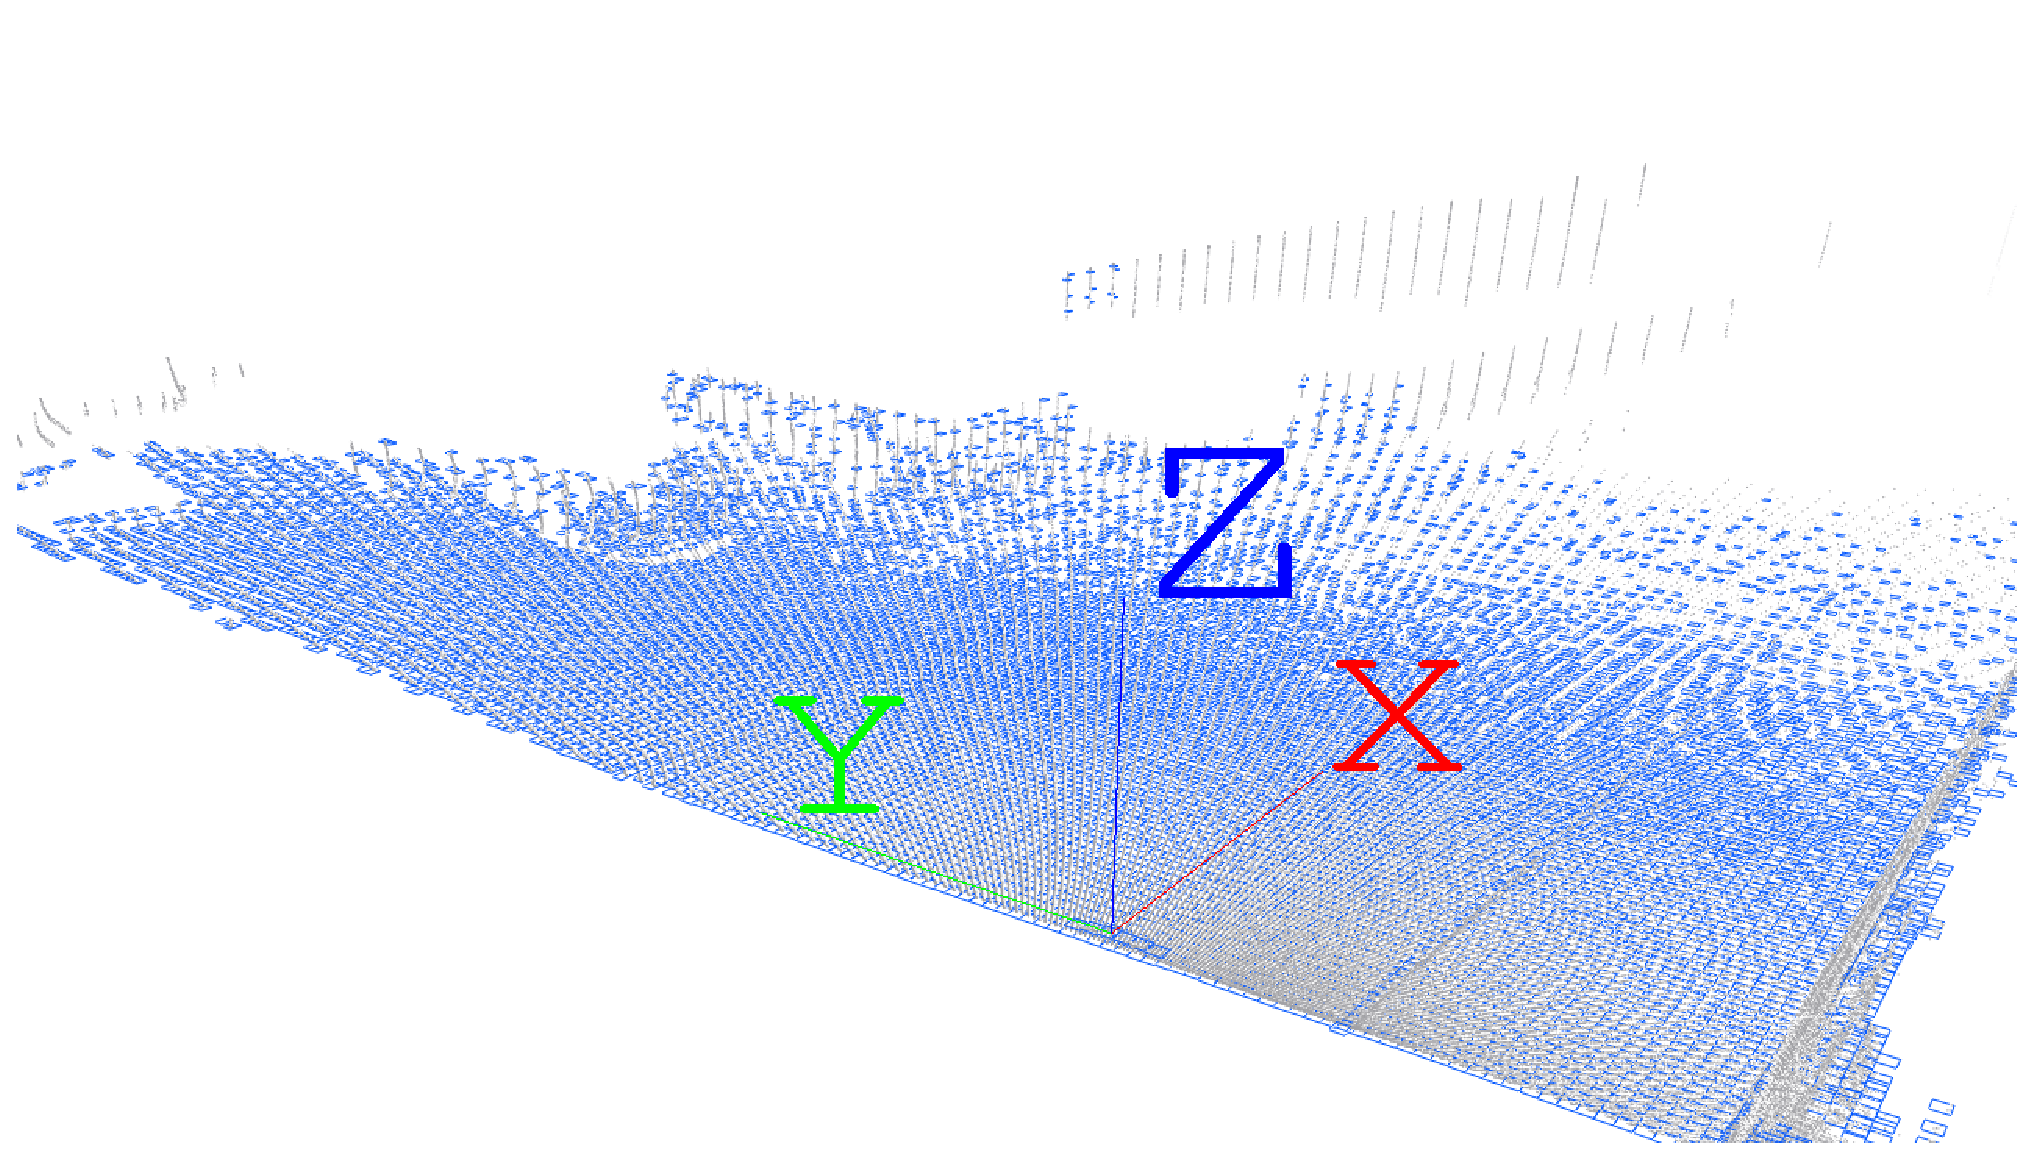
\includegraphics[width=\columnwidth]{fig/dem.eps}
\caption{DEM example from a 3D point cloud representation.}
\label{fig:dem}
\end{figure}

\subsection{Environment Model and Inference Task}
We assume a piecewise planar environment, i.e., the observed scene is composed
of a set of plane segments. Boundaries between plane segments define local
height discontinuities that we shall henceforth term \emph{curbs}.
Fig.~\ref{fig:model} depicts a typical environment model. The major
inference task therefore boils down to discovering those plane segments. To this
end, we model the environment as a \emph{mixture of linear regressions}.
According to the discussions in~\cite{bishop06pattern}, we may thus state the
following generative process for the height values:

\begin{equation}
\label{eqn:mixture}
h_i\sim p(h_i\mid\Theta)=\sum_{k=1}^K\pi_k\mathcal{N}(h_i\mid
\mathbf{w}_k^\text{T}\boldsymbol{\phi}(\mathbf{c}_i),\sigma^2_k),
\end{equation}

where $\Theta=\{\boldsymbol{\pi},\mathbf{W},\boldsymbol{\sigma}^2\}$ is the set
of adaptive parameters, $\boldsymbol{\pi}=\{\pi_k\}$ are the mixture weights,
$\mathbf{W}=\{\mathbf{w}_k\}$ the regression coefficients,
$\boldsymbol{\sigma}^2=\{\sigma^2_k\}$ the regression variances, and
$\boldsymbol{\phi}(\mathbf{c}_i)=[1,\mathbf{c}_i]^\text{T}$ is the basis
function.

\begin{figure}[t]
\centering
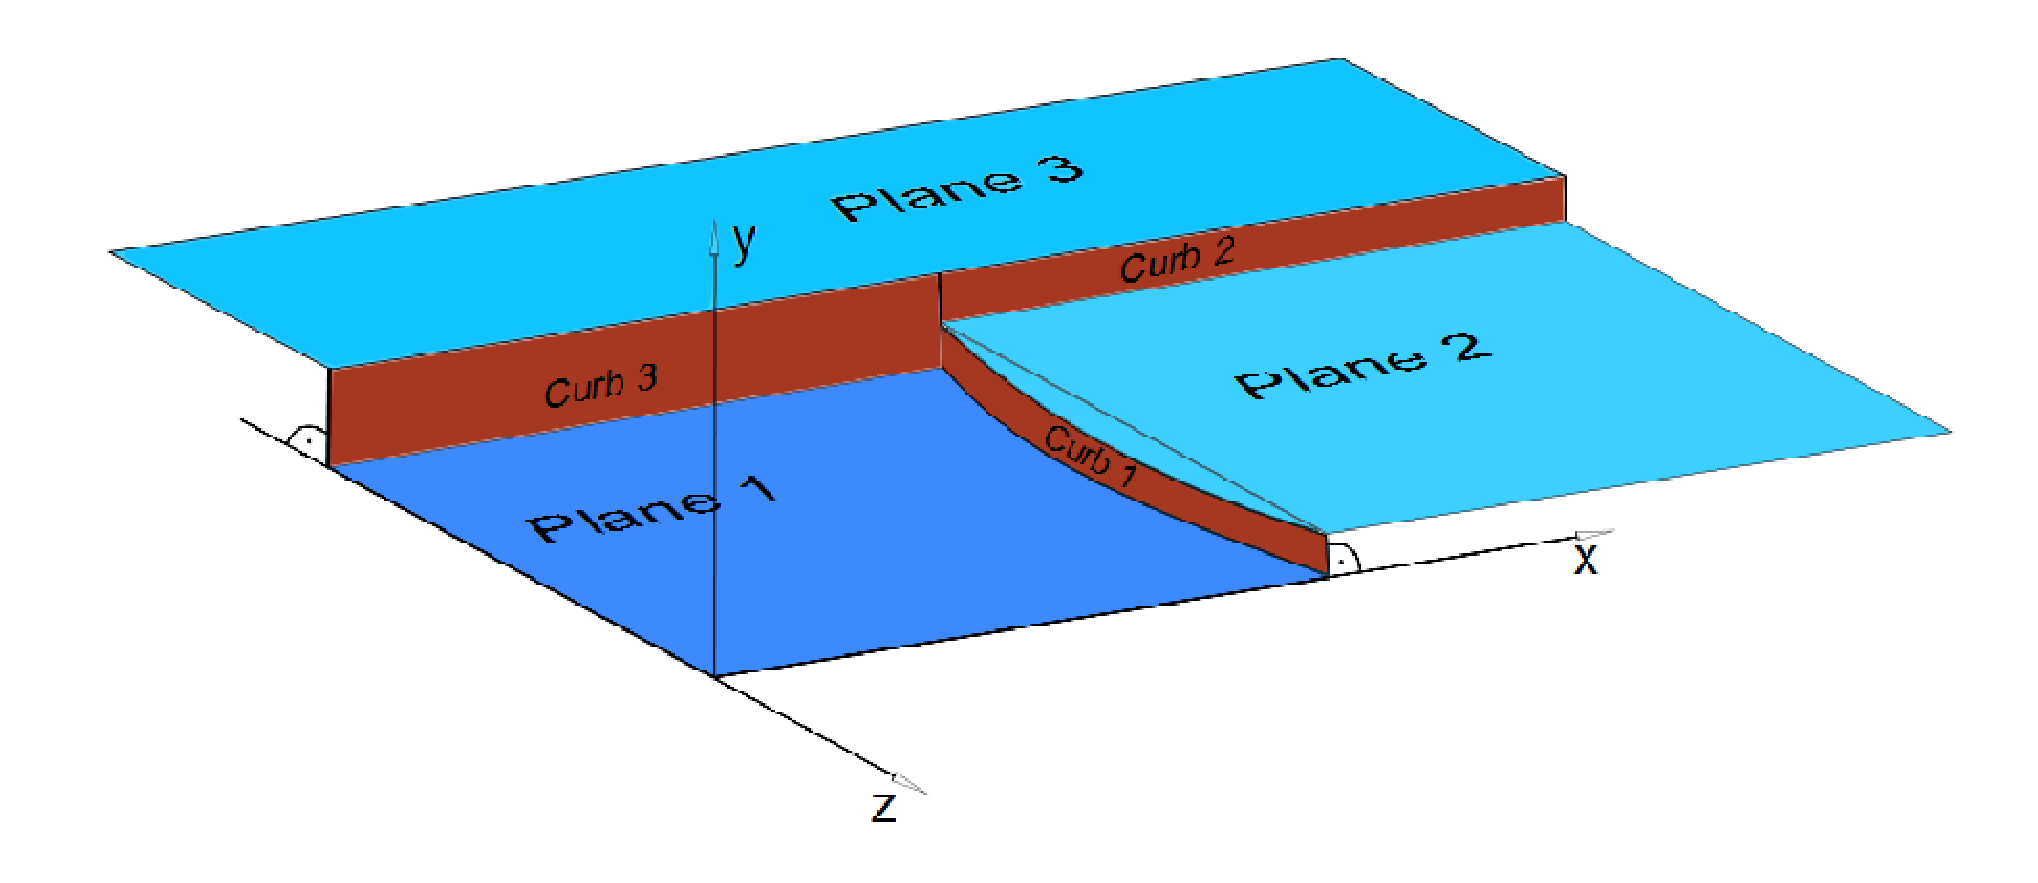
\includegraphics[width=\columnwidth]{fig/model.eps}
\caption{Typical environment model, composed of a set of plane segments. Curbs
are defined as the boundaries between plane segments.}
\label{fig:model}
\end{figure}

Similarly to Gaussian Mixture Models (GMM), one can resort to the popular
Expectation-Maximization (EM) algorithm~\cite{dempster77maximum} for estimating
the parameter set $\Theta$ given a set of observations
$\{\{h_i,\mathbf{c}_i\}\}_{i=1}^{M'}$, where $M'$ is the number of valid cells.
The algorithm alternates between the computation of \emph{responsibilities}
$\gamma_{ik}$ given an old estimate $\Theta^\text{old}$, and the computation of
$\Theta^\text{new}$ given $\gamma_{ik}$. The term $\gamma_{ik}$ can be
interpreted as the probability of a point $h_i$ belonging to a plane $k$. We
thus define the label distribution $l_i$ to be a discrete distribution with a
probability mass function $P(l_i=k)=\gamma_{ik}$.

In order to determine the number of planes $k$ and the initial responsibilities,
we apply the algorithm presented in Section~\ref{sec:initial}. The following
responsibilities are then evaluated with the Conditional Random Field (CRF) of
Section~\ref{sec:crf} and the parameter set $\Theta^\text{new}$ with the method
of Section~\ref{sec:plane}.
